\documentclass[twoside]{book}

% Packages required by doxygen
\usepackage{fixltx2e}
\usepackage{calc}
\usepackage{doxygen}
\usepackage[export]{adjustbox} % also loads graphicx
\usepackage{graphicx}
\usepackage[utf8]{inputenc}
\usepackage{makeidx}
\usepackage{multicol}
\usepackage{multirow}
\PassOptionsToPackage{warn}{textcomp}
\usepackage{textcomp}
\usepackage[nointegrals]{wasysym}
\usepackage[table]{xcolor}

% Font selection
\usepackage[T1]{fontenc}
\usepackage[scaled=.90]{helvet}
\usepackage{courier}
\usepackage{amssymb}
\usepackage{sectsty}
\renewcommand{\familydefault}{\sfdefault}
\allsectionsfont{%
  \fontseries{bc}\selectfont%
  \color{darkgray}%
}
\renewcommand{\DoxyLabelFont}{%
  \fontseries{bc}\selectfont%
  \color{darkgray}%
}
\newcommand{\+}{\discretionary{\mbox{\scriptsize$\hookleftarrow$}}{}{}}

% Page & text layout
\usepackage{geometry}
\geometry{%
  a4paper,%
  top=2.5cm,%
  bottom=2.5cm,%
  left=2.5cm,%
  right=2.5cm%
}
\tolerance=750
\hfuzz=15pt
\hbadness=750
\setlength{\emergencystretch}{15pt}
\setlength{\parindent}{0cm}
\setlength{\parskip}{3ex plus 2ex minus 2ex}
\makeatletter
\renewcommand{\paragraph}{%
  \@startsection{paragraph}{4}{0ex}{-1.0ex}{1.0ex}{%
    \normalfont\normalsize\bfseries\SS@parafont%
  }%
}
\renewcommand{\subparagraph}{%
  \@startsection{subparagraph}{5}{0ex}{-1.0ex}{1.0ex}{%
    \normalfont\normalsize\bfseries\SS@subparafont%
  }%
}
\makeatother

% Headers & footers
\usepackage{fancyhdr}
\pagestyle{fancyplain}
\fancyhead[LE]{\fancyplain{}{\bfseries\thepage}}
\fancyhead[CE]{\fancyplain{}{}}
\fancyhead[RE]{\fancyplain{}{\bfseries\leftmark}}
\fancyhead[LO]{\fancyplain{}{\bfseries\rightmark}}
\fancyhead[CO]{\fancyplain{}{}}
\fancyhead[RO]{\fancyplain{}{\bfseries\thepage}}
\fancyfoot[LE]{\fancyplain{}{}}
\fancyfoot[CE]{\fancyplain{}{}}
\fancyfoot[RE]{\fancyplain{}{\bfseries\scriptsize Generated by Doxygen }}
\fancyfoot[LO]{\fancyplain{}{\bfseries\scriptsize Generated by Doxygen }}
\fancyfoot[CO]{\fancyplain{}{}}
\fancyfoot[RO]{\fancyplain{}{}}
\renewcommand{\footrulewidth}{0.4pt}
\renewcommand{\chaptermark}[1]{%
  \markboth{#1}{}%
}
\renewcommand{\sectionmark}[1]{%
  \markright{\thesection\ #1}%
}

% Indices & bibliography
\usepackage{natbib}
\usepackage[titles]{tocloft}
\setcounter{tocdepth}{3}
\setcounter{secnumdepth}{5}
\makeindex

% Hyperlinks (required, but should be loaded last)
\usepackage{ifpdf}
\ifpdf
  \usepackage[pdftex,pagebackref=true]{hyperref}
\else
  \usepackage[ps2pdf,pagebackref=true]{hyperref}
\fi
\hypersetup{%
  colorlinks=true,%
  linkcolor=blue,%
  citecolor=blue,%
  unicode%
}

% Custom commands
\newcommand{\clearemptydoublepage}{%
  \newpage{\pagestyle{empty}\cleardoublepage}%
}

\usepackage{caption}
\captionsetup{labelsep=space,justification=centering,font={bf},singlelinecheck=off,skip=4pt,position=top}

%===== C O N T E N T S =====

\begin{document}

% Titlepage & ToC
\hypersetup{pageanchor=false,
             bookmarksnumbered=true,
             pdfencoding=unicode
            }
\pagenumbering{alph}
\begin{titlepage}
\vspace*{7cm}
\begin{center}%
{\Large My Project }\\
\vspace*{1cm}
{\large Generated by Doxygen 1.8.13}\\
\end{center}
\end{titlepage}
\clearemptydoublepage
\pagenumbering{roman}
\tableofcontents
\clearemptydoublepage
\pagenumbering{arabic}
\hypersetup{pageanchor=true}

%--- Begin generated contents ---
\chapter{Hierarchical Index}
\section{Class Hierarchy}
This inheritance list is sorted roughly, but not completely, alphabetically\+:\begin{DoxyCompactList}
\item Q\+Object\begin{DoxyCompactList}
\item \contentsline{section}{Stock\+Chart}{\pageref{class_stock_chart}}{}
\end{DoxyCompactList}
\end{DoxyCompactList}

\chapter{Class Index}
\section{Class List}
Here are the classes, structs, unions and interfaces with brief descriptions\+:\begin{DoxyCompactList}
\item\contentsline{section}{\hyperlink{class_q_t___c_h_a_r_t_s___u_s_e___n_a_m_e_s_p_a_c_e}{Q\+T\+\_\+\+C\+H\+A\+R\+T\+S\+\_\+\+U\+S\+E\+\_\+\+N\+A\+M\+E\+S\+P\+A\+CE} \\*$<$ Namespace for Qt\+Charts }{\pageref{class_q_t___c_h_a_r_t_s___u_s_e___n_a_m_e_s_p_a_c_e}}{}
\item\contentsline{section}{\hyperlink{class_stock_chart}{Stock\+Chart} }{\pageref{class_stock_chart}}{}
\end{DoxyCompactList}

\chapter{File Index}
\section{File List}
Here is a list of all documented files with brief descriptions\+:\begin{DoxyCompactList}
\item\contentsline{section}{\hyperlink{main_8cpp}{main.\+cpp} }{\pageref{main_8cpp}}{}
\item\contentsline{section}{\hyperlink{stockchart_8h}{stockchart.\+h} }{\pageref{stockchart_8h}}{}
\end{DoxyCompactList}

\chapter{Class Documentation}
\hypertarget{class_q_t___c_h_a_r_t_s___u_s_e___n_a_m_e_s_p_a_c_e}{}\section{Q\+T\+\_\+\+C\+H\+A\+R\+T\+S\+\_\+\+U\+S\+E\+\_\+\+N\+A\+M\+E\+S\+P\+A\+CE Class Reference}
\label{class_q_t___c_h_a_r_t_s___u_s_e___n_a_m_e_s_p_a_c_e}\index{Q\+T\+\_\+\+C\+H\+A\+R\+T\+S\+\_\+\+U\+S\+E\+\_\+\+N\+A\+M\+E\+S\+P\+A\+CE@{Q\+T\+\_\+\+C\+H\+A\+R\+T\+S\+\_\+\+U\+S\+E\+\_\+\+N\+A\+M\+E\+S\+P\+A\+CE}}


$<$ Namespace for Qt\+Charts  




{\ttfamily \#include $<$stockchart.\+h$>$}



\subsection{Detailed Description}
$<$ Namespace for Qt\+Charts 

The \hyperlink{class_stock_chart}{Stock\+Chart} class

A class that handles data for a Q\+ML Chart\+View type object. It extends the class Q\+Object 

The documentation for this class was generated from the following file\+:\begin{DoxyCompactItemize}
\item 
\hyperlink{stockchart_8h}{stockchart.\+h}\end{DoxyCompactItemize}

\hypertarget{class_stock_chart}{}\section{Stock\+Chart Class Reference}
\label{class_stock_chart}\index{Stock\+Chart@{Stock\+Chart}}
Inheritance diagram for Stock\+Chart\+:\begin{figure}[H]
\begin{center}
\leavevmode
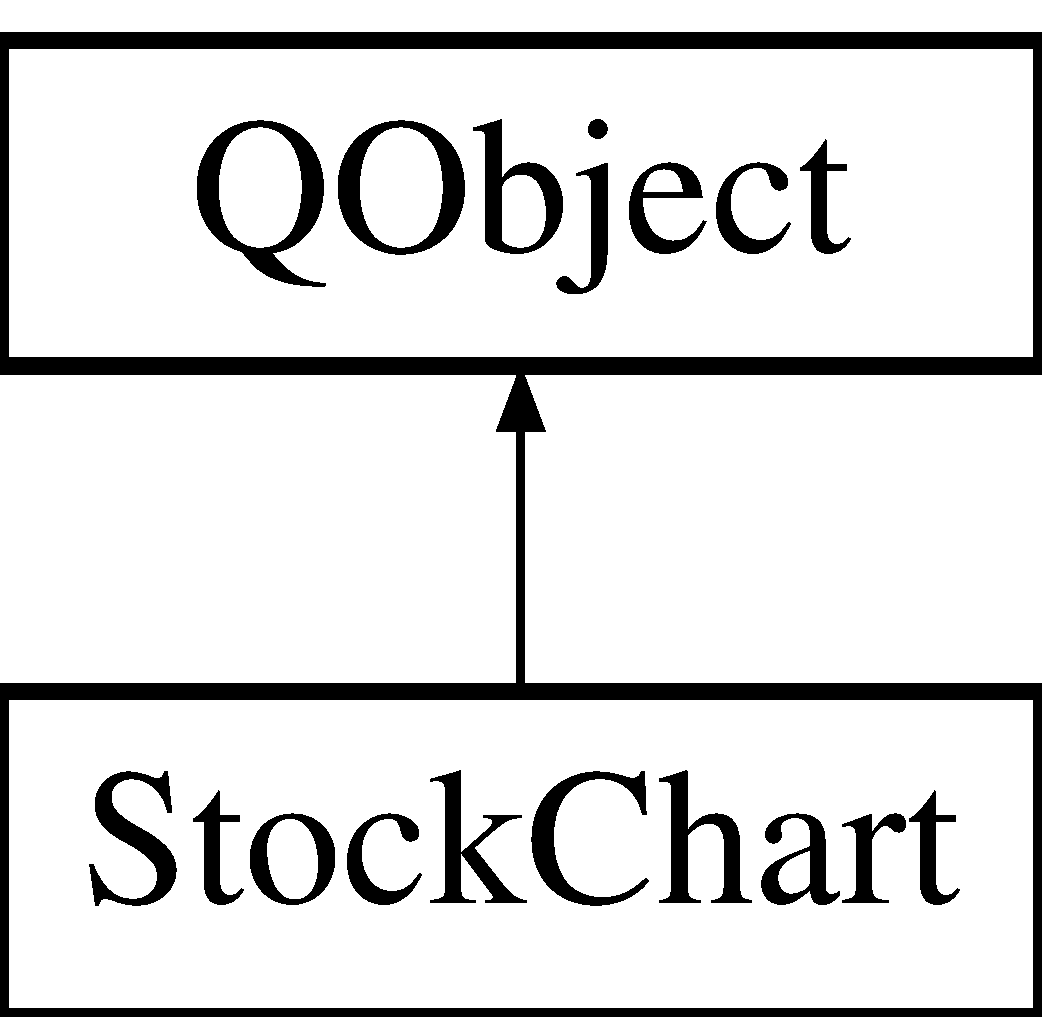
\includegraphics[height=2.000000cm]{class_stock_chart}
\end{center}
\end{figure}
\subsection*{Public Slots}
\begin{DoxyCompactItemize}
\item 
void \hyperlink{class_stock_chart_a2521c5991cca0803f5890e23d90672da}{reply\+Finished} (Q\+Network\+Reply $\ast$reply)
\begin{DoxyCompactList}\small\item\em reply\+Finished Processes the network request issued by $<$get\+Stock\+Data$>$ when the requested data is available. This function is a Qt public S\+L\+OT \end{DoxyCompactList}\end{DoxyCompactItemize}
\subsection*{Signals}
\begin{DoxyCompactItemize}
\item 
void \hyperlink{class_stock_chart_a9065188a2340a471d3db38fdd1763411}{time\+Series\+Ready} (Q\+String stock\+ID)
\begin{DoxyCompactList}\small\item\em time\+Series\+Ready Qt S\+I\+G\+N\+AL used to indicate that the time series data is ready to be added to the chart \end{DoxyCompactList}\item 
void \hyperlink{class_stock_chart_a4f0cf491de4e546621bac94bec52abc2}{start\+Date\+Changed} (const Q\+String \&date)
\begin{DoxyCompactList}\small\item\em start\+Date\+Changed Qt S\+I\+G\+N\+AL used to indicate that the X-\/axis minimum value has changed \end{DoxyCompactList}\item 
void \hyperlink{class_stock_chart_a4f7074ac61cf94ca61eb85d6869846c3}{end\+Date\+Changed} (const Q\+String \&date)
\begin{DoxyCompactList}\small\item\em end\+Date\+Changed Qt S\+I\+G\+N\+AL used to indicate that the X-\/axis maximum value has changed \end{DoxyCompactList}\item 
void \hyperlink{class_stock_chart_aefe9dfa0898e3f4daff97fe6cec674dc}{y\+Axis\+Min\+Changed} (double value)
\begin{DoxyCompactList}\small\item\em y\+Axis\+Min\+Changed Qt S\+I\+G\+N\+AL used to indicate that the Y-\/axis minimum value has changed \end{DoxyCompactList}\item 
void \hyperlink{class_stock_chart_a336420011eff34ae4b5c1afded4873db}{y\+Axis\+Max\+Changed} (double value)
\begin{DoxyCompactList}\small\item\em y\+Axis\+Max\+Changed Qt S\+I\+G\+N\+AL used to indicate that the Y-\/axis maximum value has changed \end{DoxyCompactList}\end{DoxyCompactItemize}
\subsection*{Public Member Functions}
\begin{DoxyCompactItemize}
\item 
\hyperlink{class_stock_chart_a93b8197ae88bda092ea1fd3a123ed7ea}{Stock\+Chart} (Q\+Object $\ast$parent=0)
\begin{DoxyCompactList}\small\item\em \hyperlink{class_stock_chart}{Stock\+Chart} Class Constructor -\/ Initializes a \hyperlink{class_stock_chart}{Stock\+Chart} object. \end{DoxyCompactList}\item 
Q\+String \hyperlink{class_stock_chart_a7b80ba09f101dd678db485f0ebe47c79}{start\+Date} () const
\begin{DoxyCompactList}\small\item\em start\+Date Returns the minimum date value for the chart\textquotesingle{}s X-\/axis. \end{DoxyCompactList}\item 
void \hyperlink{class_stock_chart_abf5fe9792d1587718d89892776a7ce7a}{set\+Start\+Date} (const Q\+String \&date)
\begin{DoxyCompactList}\small\item\em set\+Start\+Date Sets the minimum date value for the chart\textquotesingle{}s X-\/axis. \end{DoxyCompactList}\item 
Q\+String \hyperlink{class_stock_chart_a0c4ea05e46ed7c7b200063ec34241db1}{end\+Date} () const
\begin{DoxyCompactList}\small\item\em end\+Date Returns the maximum date value for the chart\textquotesingle{}s X-\/axis. \end{DoxyCompactList}\item 
void \hyperlink{class_stock_chart_a99d57c44a0bd5e91e2e810bec071f7db}{set\+End\+Date} (const Q\+String \&date)
\begin{DoxyCompactList}\small\item\em set\+End\+Date Sets the maximum date value for the chart\textquotesingle{}s X-\/axis. \end{DoxyCompactList}\item 
double \hyperlink{class_stock_chart_a5b03fca2a7985f4802623be2c86f1316}{y\+Axis\+Min} () const
\begin{DoxyCompactList}\small\item\em y\+Axis\+Min Returns the minimum value for the chart\textquotesingle{}s Y-\/axis. \end{DoxyCompactList}\item 
void \hyperlink{class_stock_chart_a4cfeb533f5b01e029cb25831252d8f1d}{set\+Y\+Axis\+Min} (double value)
\begin{DoxyCompactList}\small\item\em set\+Y\+Axis\+Min Sets the minimum value for the chart\textquotesingle{}s Y-\/axis. \end{DoxyCompactList}\item 
double \hyperlink{class_stock_chart_a385cf91d047bd0cad511a0e068ed239f}{y\+Axis\+Max} () const
\begin{DoxyCompactList}\small\item\em y\+Axis\+Max Returns the maximum value for the chart\textquotesingle{}s Y-\/axis. \end{DoxyCompactList}\item 
\mbox{\Hypertarget{class_stock_chart_aeedaaefe37da9b061e2cf4f8a618b7c1}\label{class_stock_chart_aeedaaefe37da9b061e2cf4f8a618b7c1}} 
void \hyperlink{class_stock_chart_aeedaaefe37da9b061e2cf4f8a618b7c1}{set\+Y\+Axis\+Max} (double value)
\begin{DoxyCompactList}\small\item\em set\+Y\+Axis\+Max Sets the maximum value for the chart\textquotesingle{}s Y-\/axis. \end{DoxyCompactList}\item 
Q\+\_\+\+I\+N\+V\+O\+K\+A\+B\+LE void \hyperlink{class_stock_chart_a263508e678183faf4ce6a98ecab71405}{set\+Line\+Series} (Q\+Line\+Series $\ast$line\+Series)
\begin{DoxyCompactList}\small\item\em set\+Line\+Series Creates the data to be shown in the chart. This data corresponds to one line plot or line series in the chart. This function can be called from a Q\+ML file since it is marked as Q\+\_\+\+I\+N\+V\+O\+K\+A\+B\+LE. \end{DoxyCompactList}\item 
Q\+\_\+\+I\+N\+V\+O\+K\+A\+B\+LE void \hyperlink{class_stock_chart_ab108485d635146b2dc9bb1192c4371ec}{get\+Stock\+Data} (const Q\+String \&stock\+ID)
\begin{DoxyCompactList}\small\item\em get\+Stock\+Data Sends/issues a network request to fetch the data for a particular financial instrument / security / stock from the internet \href{https://www.alphavantage.co/}{\tt https\+://www.\+alphavantage.\+co/}. The data fetched is a time series \href{https://en.wikipedia.org/wiki/Time_series}{\tt https\+://en.\+wikipedia.\+org/wiki/\+Time\+\_\+series}. This function can be called from a Q\+ML file since it is marked as Q\+\_\+\+I\+N\+V\+O\+K\+A\+B\+LE. \end{DoxyCompactList}\end{DoxyCompactItemize}
\subsection*{Properties}
\begin{DoxyCompactItemize}
\item 
\mbox{\Hypertarget{class_stock_chart_add7099e870c86ce5a1c9ba88bced379c}\label{class_stock_chart_add7099e870c86ce5a1c9ba88bced379c}} 
Q\+String {\bfseries start\+Date}
\item 
\mbox{\Hypertarget{class_stock_chart_aab43c54ca8f5aafcb68170b7684775f4}\label{class_stock_chart_aab43c54ca8f5aafcb68170b7684775f4}} 
Q\+String {\bfseries end\+Date}
\item 
\mbox{\Hypertarget{class_stock_chart_ae2c25f0548c61c72c2467b4bbf519a09}\label{class_stock_chart_ae2c25f0548c61c72c2467b4bbf519a09}} 
double {\bfseries y\+Axis\+Min}
\item 
\mbox{\Hypertarget{class_stock_chart_a77e182d1098f84f08bbd23bd0e2dbf9a}\label{class_stock_chart_a77e182d1098f84f08bbd23bd0e2dbf9a}} 
double {\bfseries y\+Axis\+Max}
\end{DoxyCompactItemize}


\subsection{Constructor \& Destructor Documentation}
\mbox{\Hypertarget{class_stock_chart_a93b8197ae88bda092ea1fd3a123ed7ea}\label{class_stock_chart_a93b8197ae88bda092ea1fd3a123ed7ea}} 
\index{Stock\+Chart@{Stock\+Chart}!Stock\+Chart@{Stock\+Chart}}
\index{Stock\+Chart@{Stock\+Chart}!Stock\+Chart@{Stock\+Chart}}
\subsubsection{\texorpdfstring{Stock\+Chart()}{StockChart()}}
{\footnotesize\ttfamily Stock\+Chart\+::\+Stock\+Chart (\begin{DoxyParamCaption}\item[{Q\+Object $\ast$}]{parent = {\ttfamily 0} }\end{DoxyParamCaption})\hspace{0.3cm}{\ttfamily [explicit]}}



\hyperlink{class_stock_chart}{Stock\+Chart} Class Constructor -\/ Initializes a \hyperlink{class_stock_chart}{Stock\+Chart} object. 


\begin{DoxyParams}{Parameters}
{\em parent} & Q\+Object \\
\hline
\end{DoxyParams}


\subsection{Member Function Documentation}
\mbox{\Hypertarget{class_stock_chart_a0c4ea05e46ed7c7b200063ec34241db1}\label{class_stock_chart_a0c4ea05e46ed7c7b200063ec34241db1}} 
\index{Stock\+Chart@{Stock\+Chart}!end\+Date@{end\+Date}}
\index{end\+Date@{end\+Date}!Stock\+Chart@{Stock\+Chart}}
\subsubsection{\texorpdfstring{end\+Date()}{endDate()}}
{\footnotesize\ttfamily Q\+String Stock\+Chart\+::end\+Date (\begin{DoxyParamCaption}{ }\end{DoxyParamCaption}) const}



end\+Date Returns the maximum date value for the chart\textquotesingle{}s X-\/axis. 

\begin{DoxyReturn}{Returns}
Returns the maximum date value for the chart\textquotesingle{}s X-\/axis. 
\end{DoxyReturn}
\mbox{\Hypertarget{class_stock_chart_a4f7074ac61cf94ca61eb85d6869846c3}\label{class_stock_chart_a4f7074ac61cf94ca61eb85d6869846c3}} 
\index{Stock\+Chart@{Stock\+Chart}!end\+Date\+Changed@{end\+Date\+Changed}}
\index{end\+Date\+Changed@{end\+Date\+Changed}!Stock\+Chart@{Stock\+Chart}}
\subsubsection{\texorpdfstring{end\+Date\+Changed}{endDateChanged}}
{\footnotesize\ttfamily void Stock\+Chart\+::end\+Date\+Changed (\begin{DoxyParamCaption}\item[{const Q\+String \&}]{date }\end{DoxyParamCaption})\hspace{0.3cm}{\ttfamily [signal]}}



end\+Date\+Changed Qt S\+I\+G\+N\+AL used to indicate that the X-\/axis maximum value has changed 


\begin{DoxyParams}{Parameters}
{\em date} & Value to which m\+\_\+\+End\+Date \& end\+Date were changed \\
\hline
\end{DoxyParams}
\mbox{\Hypertarget{class_stock_chart_ab108485d635146b2dc9bb1192c4371ec}\label{class_stock_chart_ab108485d635146b2dc9bb1192c4371ec}} 
\index{Stock\+Chart@{Stock\+Chart}!get\+Stock\+Data@{get\+Stock\+Data}}
\index{get\+Stock\+Data@{get\+Stock\+Data}!Stock\+Chart@{Stock\+Chart}}
\subsubsection{\texorpdfstring{get\+Stock\+Data()}{getStockData()}}
{\footnotesize\ttfamily void Stock\+Chart\+::get\+Stock\+Data (\begin{DoxyParamCaption}\item[{const Q\+String \&}]{stock\+ID }\end{DoxyParamCaption})}



get\+Stock\+Data Sends/issues a network request to fetch the data for a particular financial instrument / security / stock from the internet \href{https://www.alphavantage.co/}{\tt https\+://www.\+alphavantage.\+co/}. The data fetched is a time series \href{https://en.wikipedia.org/wiki/Time_series}{\tt https\+://en.\+wikipedia.\+org/wiki/\+Time\+\_\+series}. This function can be called from a Q\+ML file since it is marked as Q\+\_\+\+I\+N\+V\+O\+K\+A\+B\+LE. 


\begin{DoxyParams}{Parameters}
{\em stock\+ID} & String with the Ticker Symbol or ID assigned to a particular security / stock that is to be fetched from the internet \\
\hline
\end{DoxyParams}
\mbox{\Hypertarget{class_stock_chart_a2521c5991cca0803f5890e23d90672da}\label{class_stock_chart_a2521c5991cca0803f5890e23d90672da}} 
\index{Stock\+Chart@{Stock\+Chart}!reply\+Finished@{reply\+Finished}}
\index{reply\+Finished@{reply\+Finished}!Stock\+Chart@{Stock\+Chart}}
\subsubsection{\texorpdfstring{reply\+Finished}{replyFinished}}
{\footnotesize\ttfamily void Stock\+Chart\+::reply\+Finished (\begin{DoxyParamCaption}\item[{Q\+Network\+Reply $\ast$}]{reply }\end{DoxyParamCaption})\hspace{0.3cm}{\ttfamily [slot]}}



reply\+Finished Processes the network request issued by $<$get\+Stock\+Data$>$ when the requested data is available. This function is a Qt public S\+L\+OT 


\begin{DoxyParams}{Parameters}
{\em reply} & Pointer to a Q\+Network\+Reply object that contains the requested network data \\
\hline
\end{DoxyParams}
\mbox{\Hypertarget{class_stock_chart_a99d57c44a0bd5e91e2e810bec071f7db}\label{class_stock_chart_a99d57c44a0bd5e91e2e810bec071f7db}} 
\index{Stock\+Chart@{Stock\+Chart}!set\+End\+Date@{set\+End\+Date}}
\index{set\+End\+Date@{set\+End\+Date}!Stock\+Chart@{Stock\+Chart}}
\subsubsection{\texorpdfstring{set\+End\+Date()}{setEndDate()}}
{\footnotesize\ttfamily void Stock\+Chart\+::set\+End\+Date (\begin{DoxyParamCaption}\item[{const Q\+String \&}]{date }\end{DoxyParamCaption})}



set\+End\+Date Sets the maximum date value for the chart\textquotesingle{}s X-\/axis. 


\begin{DoxyParams}{Parameters}
{\em date} & \\
\hline
\end{DoxyParams}
\mbox{\Hypertarget{class_stock_chart_a263508e678183faf4ce6a98ecab71405}\label{class_stock_chart_a263508e678183faf4ce6a98ecab71405}} 
\index{Stock\+Chart@{Stock\+Chart}!set\+Line\+Series@{set\+Line\+Series}}
\index{set\+Line\+Series@{set\+Line\+Series}!Stock\+Chart@{Stock\+Chart}}
\subsubsection{\texorpdfstring{set\+Line\+Series()}{setLineSeries()}}
{\footnotesize\ttfamily void Stock\+Chart\+::set\+Line\+Series (\begin{DoxyParamCaption}\item[{Q\+Line\+Series $\ast$}]{line\+Series }\end{DoxyParamCaption})}



set\+Line\+Series Creates the data to be shown in the chart. This data corresponds to one line plot or line series in the chart. This function can be called from a Q\+ML file since it is marked as Q\+\_\+\+I\+N\+V\+O\+K\+A\+B\+LE. 


\begin{DoxyParams}{Parameters}
{\em line\+Series} & -\/ Pointer to a Q\+Line\+Series object that belongs to the Q\+ML chart (Chart\+View) and needs to be filled with valid data in order to be displayed as a line plot in the chart \\
\hline
\end{DoxyParams}
\mbox{\Hypertarget{class_stock_chart_abf5fe9792d1587718d89892776a7ce7a}\label{class_stock_chart_abf5fe9792d1587718d89892776a7ce7a}} 
\index{Stock\+Chart@{Stock\+Chart}!set\+Start\+Date@{set\+Start\+Date}}
\index{set\+Start\+Date@{set\+Start\+Date}!Stock\+Chart@{Stock\+Chart}}
\subsubsection{\texorpdfstring{set\+Start\+Date()}{setStartDate()}}
{\footnotesize\ttfamily void Stock\+Chart\+::set\+Start\+Date (\begin{DoxyParamCaption}\item[{const Q\+String \&}]{date }\end{DoxyParamCaption})}



set\+Start\+Date Sets the minimum date value for the chart\textquotesingle{}s X-\/axis. 


\begin{DoxyParams}{Parameters}
{\em date} & Value to be used as start\+Date \\
\hline
\end{DoxyParams}
\mbox{\Hypertarget{class_stock_chart_a4cfeb533f5b01e029cb25831252d8f1d}\label{class_stock_chart_a4cfeb533f5b01e029cb25831252d8f1d}} 
\index{Stock\+Chart@{Stock\+Chart}!set\+Y\+Axis\+Min@{set\+Y\+Axis\+Min}}
\index{set\+Y\+Axis\+Min@{set\+Y\+Axis\+Min}!Stock\+Chart@{Stock\+Chart}}
\subsubsection{\texorpdfstring{set\+Y\+Axis\+Min()}{setYAxisMin()}}
{\footnotesize\ttfamily void Stock\+Chart\+::set\+Y\+Axis\+Min (\begin{DoxyParamCaption}\item[{double}]{value }\end{DoxyParamCaption})}



set\+Y\+Axis\+Min Sets the minimum value for the chart\textquotesingle{}s Y-\/axis. 


\begin{DoxyParams}{Parameters}
{\em value} & \\
\hline
\end{DoxyParams}
\mbox{\Hypertarget{class_stock_chart_a7b80ba09f101dd678db485f0ebe47c79}\label{class_stock_chart_a7b80ba09f101dd678db485f0ebe47c79}} 
\index{Stock\+Chart@{Stock\+Chart}!start\+Date@{start\+Date}}
\index{start\+Date@{start\+Date}!Stock\+Chart@{Stock\+Chart}}
\subsubsection{\texorpdfstring{start\+Date()}{startDate()}}
{\footnotesize\ttfamily Q\+String Stock\+Chart\+::start\+Date (\begin{DoxyParamCaption}{ }\end{DoxyParamCaption}) const}



start\+Date Returns the minimum date value for the chart\textquotesingle{}s X-\/axis. 

\begin{DoxyReturn}{Returns}
Returns a string with the minimum date value for the chart\textquotesingle{}s X-\/axis. 
\end{DoxyReturn}
\mbox{\Hypertarget{class_stock_chart_a4f0cf491de4e546621bac94bec52abc2}\label{class_stock_chart_a4f0cf491de4e546621bac94bec52abc2}} 
\index{Stock\+Chart@{Stock\+Chart}!start\+Date\+Changed@{start\+Date\+Changed}}
\index{start\+Date\+Changed@{start\+Date\+Changed}!Stock\+Chart@{Stock\+Chart}}
\subsubsection{\texorpdfstring{start\+Date\+Changed}{startDateChanged}}
{\footnotesize\ttfamily void Stock\+Chart\+::start\+Date\+Changed (\begin{DoxyParamCaption}\item[{const Q\+String \&}]{date }\end{DoxyParamCaption})\hspace{0.3cm}{\ttfamily [signal]}}



start\+Date\+Changed Qt S\+I\+G\+N\+AL used to indicate that the X-\/axis minimum value has changed 


\begin{DoxyParams}{Parameters}
{\em date} & Value to which m\+\_\+\+Start\+Date \& start\+Date were changed \\
\hline
\end{DoxyParams}
\mbox{\Hypertarget{class_stock_chart_a9065188a2340a471d3db38fdd1763411}\label{class_stock_chart_a9065188a2340a471d3db38fdd1763411}} 
\index{Stock\+Chart@{Stock\+Chart}!time\+Series\+Ready@{time\+Series\+Ready}}
\index{time\+Series\+Ready@{time\+Series\+Ready}!Stock\+Chart@{Stock\+Chart}}
\subsubsection{\texorpdfstring{time\+Series\+Ready}{timeSeriesReady}}
{\footnotesize\ttfamily void Stock\+Chart\+::time\+Series\+Ready (\begin{DoxyParamCaption}\item[{Q\+String}]{stock\+ID }\end{DoxyParamCaption})\hspace{0.3cm}{\ttfamily [signal]}}



time\+Series\+Ready Qt S\+I\+G\+N\+AL used to indicate that the time series data is ready to be added to the chart 


\begin{DoxyParams}{Parameters}
{\em stock\+ID} & \\
\hline
\end{DoxyParams}
\mbox{\Hypertarget{class_stock_chart_a385cf91d047bd0cad511a0e068ed239f}\label{class_stock_chart_a385cf91d047bd0cad511a0e068ed239f}} 
\index{Stock\+Chart@{Stock\+Chart}!y\+Axis\+Max@{y\+Axis\+Max}}
\index{y\+Axis\+Max@{y\+Axis\+Max}!Stock\+Chart@{Stock\+Chart}}
\subsubsection{\texorpdfstring{y\+Axis\+Max()}{yAxisMax()}}
{\footnotesize\ttfamily double Stock\+Chart\+::y\+Axis\+Max (\begin{DoxyParamCaption}{ }\end{DoxyParamCaption}) const}



y\+Axis\+Max Returns the maximum value for the chart\textquotesingle{}s Y-\/axis. 

\begin{DoxyReturn}{Returns}
Returns the maximum value for the chart\textquotesingle{}s Y-\/axis. 
\end{DoxyReturn}
\mbox{\Hypertarget{class_stock_chart_a336420011eff34ae4b5c1afded4873db}\label{class_stock_chart_a336420011eff34ae4b5c1afded4873db}} 
\index{Stock\+Chart@{Stock\+Chart}!y\+Axis\+Max\+Changed@{y\+Axis\+Max\+Changed}}
\index{y\+Axis\+Max\+Changed@{y\+Axis\+Max\+Changed}!Stock\+Chart@{Stock\+Chart}}
\subsubsection{\texorpdfstring{y\+Axis\+Max\+Changed}{yAxisMaxChanged}}
{\footnotesize\ttfamily void Stock\+Chart\+::y\+Axis\+Max\+Changed (\begin{DoxyParamCaption}\item[{double}]{value }\end{DoxyParamCaption})\hspace{0.3cm}{\ttfamily [signal]}}



y\+Axis\+Max\+Changed Qt S\+I\+G\+N\+AL used to indicate that the Y-\/axis maximum value has changed 


\begin{DoxyParams}{Parameters}
{\em value} & Value to which m\+\_\+\+Y\+Axis\+Max\& y\+Axis\+Max were changed \\
\hline
\end{DoxyParams}
\mbox{\Hypertarget{class_stock_chart_a5b03fca2a7985f4802623be2c86f1316}\label{class_stock_chart_a5b03fca2a7985f4802623be2c86f1316}} 
\index{Stock\+Chart@{Stock\+Chart}!y\+Axis\+Min@{y\+Axis\+Min}}
\index{y\+Axis\+Min@{y\+Axis\+Min}!Stock\+Chart@{Stock\+Chart}}
\subsubsection{\texorpdfstring{y\+Axis\+Min()}{yAxisMin()}}
{\footnotesize\ttfamily double Stock\+Chart\+::y\+Axis\+Min (\begin{DoxyParamCaption}{ }\end{DoxyParamCaption}) const}



y\+Axis\+Min Returns the minimum value for the chart\textquotesingle{}s Y-\/axis. 

\begin{DoxyReturn}{Returns}
Returns the minimum value for the chart\textquotesingle{}s Y-\/axis. 
\end{DoxyReturn}
\mbox{\Hypertarget{class_stock_chart_aefe9dfa0898e3f4daff97fe6cec674dc}\label{class_stock_chart_aefe9dfa0898e3f4daff97fe6cec674dc}} 
\index{Stock\+Chart@{Stock\+Chart}!y\+Axis\+Min\+Changed@{y\+Axis\+Min\+Changed}}
\index{y\+Axis\+Min\+Changed@{y\+Axis\+Min\+Changed}!Stock\+Chart@{Stock\+Chart}}
\subsubsection{\texorpdfstring{y\+Axis\+Min\+Changed}{yAxisMinChanged}}
{\footnotesize\ttfamily void Stock\+Chart\+::y\+Axis\+Min\+Changed (\begin{DoxyParamCaption}\item[{double}]{value }\end{DoxyParamCaption})\hspace{0.3cm}{\ttfamily [signal]}}



y\+Axis\+Min\+Changed Qt S\+I\+G\+N\+AL used to indicate that the Y-\/axis minimum value has changed 


\begin{DoxyParams}{Parameters}
{\em value} & Value to which m\+\_\+\+Y\+Axis\+Min \& y\+Axis\+Min were changed \\
\hline
\end{DoxyParams}


The documentation for this class was generated from the following files\+:\begin{DoxyCompactItemize}
\item 
\hyperlink{stockchart_8h}{stockchart.\+h}\item 
stockchart.\+cpp\end{DoxyCompactItemize}

\chapter{File Documentation}
\hypertarget{main_8cpp}{}\section{main.\+cpp File Reference}
\label{main_8cpp}\index{main.\+cpp@{main.\+cpp}}


This file contains the \char`\"{}main\char`\"{} function. Inside, the class \hyperlink{class_stock_chart}{Stock\+Chart} is registered as a Q\+ML type object for it can be used inside a Q\+ML file.  


{\ttfamily \#include $<$Qt\+Widgets/\+Q\+Main\+Window$>$}\newline
{\ttfamily \#include $<$Q\+Qml\+Engine$>$}\newline
{\ttfamily \#include $<$Q\+Qml\+Component$>$}\newline
{\ttfamily \#include $<$Q\+Qml\+Application\+Engine$>$}\newline
{\ttfamily \#include $<$Q\+Quick\+View$>$}\newline
{\ttfamily \#include $<$Q\+Application$>$}\newline
{\ttfamily \#include \char`\"{}stockchart.\+h\char`\"{}}\newline
\subsection*{Functions}
\begin{DoxyCompactItemize}
\item 
int \hyperlink{main_8cpp_a0ddf1224851353fc92bfbff6f499fa97}{main} (int argc, char $\ast$argv\mbox{[}$\,$\mbox{]})
\begin{DoxyCompactList}\small\item\em q\+Main Entry point of A\+NY C++ program \end{DoxyCompactList}\end{DoxyCompactItemize}


\subsection{Detailed Description}
This file contains the \char`\"{}main\char`\"{} function. Inside, the class \hyperlink{class_stock_chart}{Stock\+Chart} is registered as a Q\+ML type object for it can be used inside a Q\+ML file. 



\subsection{Function Documentation}
\mbox{\Hypertarget{main_8cpp_a0ddf1224851353fc92bfbff6f499fa97}\label{main_8cpp_a0ddf1224851353fc92bfbff6f499fa97}} 
\index{main.\+cpp@{main.\+cpp}!main@{main}}
\index{main@{main}!main.\+cpp@{main.\+cpp}}
\subsubsection{\texorpdfstring{main()}{main()}}
{\footnotesize\ttfamily int main (\begin{DoxyParamCaption}\item[{int}]{argc,  }\item[{char $\ast$}]{argv\mbox{[}$\,$\mbox{]} }\end{DoxyParamCaption})}



q\+Main Entry point of A\+NY C++ program 


\begin{DoxyParams}{Parameters}
{\em argc} & Number of arguments passed to the function \\
\hline
{\em argv} & Argument vector/strings that were passed to the function \\
\hline
\end{DoxyParams}
\begin{DoxyReturn}{Returns}
app.\+exec() causes the actual application to run in an endless loop 
\end{DoxyReturn}

\hypertarget{stockchart_8h}{}\section{stockchart.\+h File Reference}
\label{stockchart_8h}\index{stockchart.\+h@{stockchart.\+h}}


\hyperlink{class_stock_chart}{Stock\+Chart} class file.  


{\ttfamily \#include $<$Qt\+Charts/\+Q\+Chart\+View$>$}\newline
{\ttfamily \#include $<$Qt\+Charts/\+Q\+Line\+Series$>$}\newline
{\ttfamily \#include $<$Qt\+Charts/\+Q\+Date\+Time\+Axis$>$}\newline
{\ttfamily \#include $<$Qt\+Charts/\+Q\+Category\+Axis$>$}\newline
{\ttfamily \#include $<$Q\+Date\+Time$>$}\newline
{\ttfamily \#include $<$Qt\+Quick/\+Q\+Quick\+Painted\+Item$>$}\newline
{\ttfamily \#include $<$Q\+Color$>$}\newline
{\ttfamily \#include $<$Q\+Object$>$}\newline
{\ttfamily \#include $<$Qt\+Network$>$}\newline
{\ttfamily \#include $<$Qt\+Core$>$}\newline
\subsection*{Classes}
\begin{DoxyCompactItemize}
\item 
class \hyperlink{class_stock_chart}{Stock\+Chart}
\begin{DoxyCompactList}\small\item\em Class \hyperlink{class_stock_chart}{Stock\+Chart}. Extends Q\+Object. \end{DoxyCompactList}\end{DoxyCompactItemize}


\subsection{Detailed Description}
\hyperlink{class_stock_chart}{Stock\+Chart} class file. 


%--- End generated contents ---

% Index
\backmatter
\newpage
\phantomsection
\clearemptydoublepage
\addcontentsline{toc}{chapter}{Index}
\printindex

\end{document}
